\documentclass{article}
\usepackage{graphicx}
\usepackage{chemformula}
\usepackage{chemmacros}
\usepackage[affil-it]{authblk}

\begin{document}

\title{Collagen Fiber Extraction and Analysis in the H\&E Dyed Cancer Tissue Images}
\author{Marius Latinis, marius.latinis@mf.stud.vu.lt \\
        Mindaugas Mork\=unas, mindaugas.morkunas@mif.vu.lt \\
        Povilas Treigys, povilas.treigys@mif.vu.lt}
\affil{Institude of Data Science and Digital Technologies, Vilnius University,
       Akademijos str. 4, Vilnius, Lithuania
}


\maketitle

\begin{abstract}
    This paper investigates the use of artificial intelligence for
    predicting cancer patients diagnosis from collagen fibers located in the digital
    Hematoxylin and Eosin stained tissue images. The proposed technique uses a convolutional
    neural network to extract a collagen mask from the image. The collagen mask is then fed
    into a second pipeline that predicts the diagnosis. We conclude that this method is
    not sufficient to generate a meaningful prediction. \\

    \textbf{keywords:} Convolutional Neural Network, Collagen Fibers.
\end{abstract}


\section{Introduction}

Visual examination of a tissue is a major part in cancer diagnosis. A
trained pathologist is given a sample of a tissue to inspect. By looking at the tissue placed
under a microscope or inspecting its digital image a pathologist diagnoses the severity of
cancer and makes a prediction about the further treatment. Unfortunatelly, manual inspection is
prone to error and inter-observer variability (e.g. different pathologists are trained
differently). This creates an interest to investigate whether a computer can perform the
tissue inspection and provide predictions.

Different components of the tissue must be coloured with different colours
so that the visual image of a tissue can be analysed. Hematoxylin and eosin
stain (abbreviated as H\&E [1]) is one of the principal tissue stains used
in histology: \\

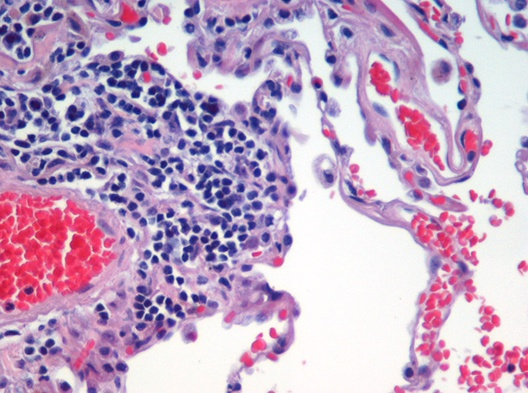
\includegraphics[width=7cm]{images/example.jpg}

The hematoxylin stains cell nuclei blue whereas eosin
stains the extracellular matrix pink, with other structures taking on
different shades, hues and combinations of these colors. The stain shows
the general layout and distribution of cells and provides a general
overview of a tissue sample's structure. It is the most widely used stain
in medical diagnosis. When a pathologist looks at a biopsy of a suspected
cancer, the histological section is likely to be stained with H\&E.

Collagen is one particular component of a tissue. It is a protein located
in the extracellular matrix, which becomes pink after the H\&E staining.
It is believed that the metastatic tumor cells interact with oriented
collagen fibers to invade the blood vessels. Several studies have shown a link between
collagen remodeling and the invasion and progression of mammary cancer in mouse
models [2,3,4]. Furthermore, there was a link observed between collagen morphology,
particularly collagen alignment, and breast cancer patient outcome [5]. Provenzano et al.[2]
first introduced the so called tumor associated collagen signature (TACS) nomenclature to
describe collagen alignment patterns. The TACS phenotypes are currently classified into three
groups. TACS-1 describes the standard desmoplastic response of increased collagen deposition
surrounding initiating tumor cells. TACS-2 is observed as straightened fibers aligned
tangentially around developing tumors. The image is considered to be TAC-3 positive if
it contains many straight collagen fibers aligned normally to the epithelial cells boundary
regions: [6] \\

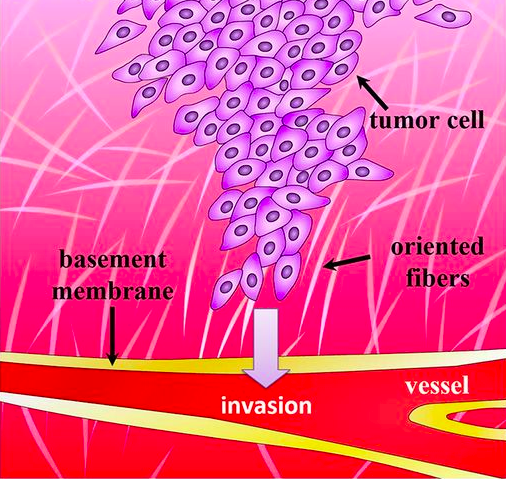
\includegraphics[width=7cm]{images/tac3.png}

Thus, collagen fibers organisation in the tissue could be used as a biomarker
to diagnose the patients cancer severity.

Previous collagen alignment studies were either carried manually, or automated on other imaging
techniques, such as the second harmonic generation (SHG) microscopy [7]. However, until the start
of this project there was no study that would implement a fully automated pipeline using solely
the H\&E stained images. This project aims to automate collagen as a biomarker extraction and
assesment procedures on the most popular H\&E stain.

\section{Methods}

\subsection{Collagen Extraction}

The first step in this project is to take the H\&E stained image containing
all tissue components and extract only the shape of a collagen present
in the image. This is known as the image segmentation problem. In this case
a pixel representing the collagen will be labelled as a foreground (bit with value 1),
whereas any other pixel will be labelled as a background (bit with value 0). Machine learning
was used to solve this problem. A model is created and provided with the training data.
The model learns to separate pixels into collagen and background classes
and can be applied to unseen images. The training data was provided by the National Center of
Pathology, Vilnius. Large H\&E images were tiled into tiles of $256 \times 256$ pixels and for
each tile a collagen mask was manually extracted with a paint software: \\

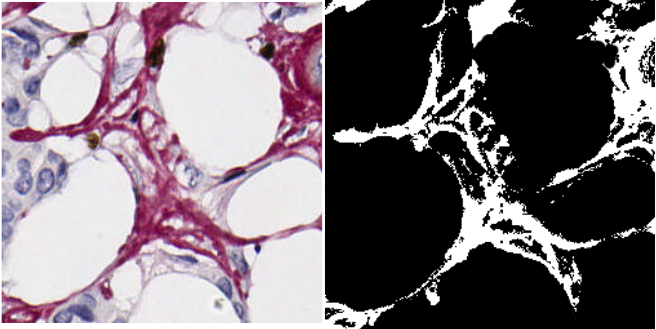
\includegraphics[width=7cm]{images/pair.png}

In total 43 image-mask pairs were used to train the model. A convolutional neural network U-net
was chosen as a model [8]. The model takes a full $256 \times 256$ (x3 for each of the RGB colour)
image as an input and performs a few downsampling procedures to infer the
deep features from the image. Each downsampled layer is then upsampled and
connected to the layer above to apply the inferred features on the image.
Eventually the model predicts the $256 \times 256$ mask. 
We tried to construct the network with different depth (i.e. the number of downsampling layers).
We found that for $256 \times 256$ size images a data generated in the 5-th and deeper layers
becomes redundant. Thus, a U-net with 4 layers was chosen as the final neural network for the
collagen segmentation problem: \\

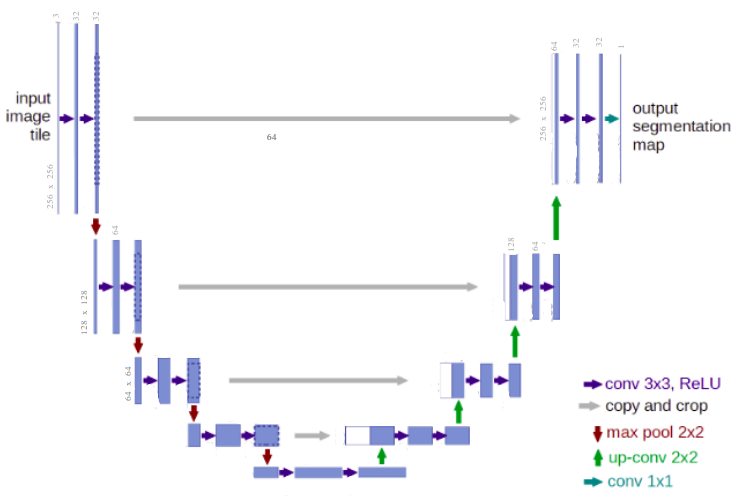
\includegraphics[width=\textwidth]{images/unet.png}

The neural network was trained on the 43 image-mask pairs using the
cross-validation technique. Binary crossentropy was used as a loss function.
Accuracy (i.e. proportion of correct foreground / background pixels) metric
was used to test the model. All code was written in python using Keras
neural network API [9]. After the model was trained, it was applied on a new
larger scale image to test its validity. The larger image was divided
into $256 \times 256$ tiles and the model was applied to each tile to extract
a collagen mask. The extracted masks were then merged into a large mask to obtain the
following result: \\

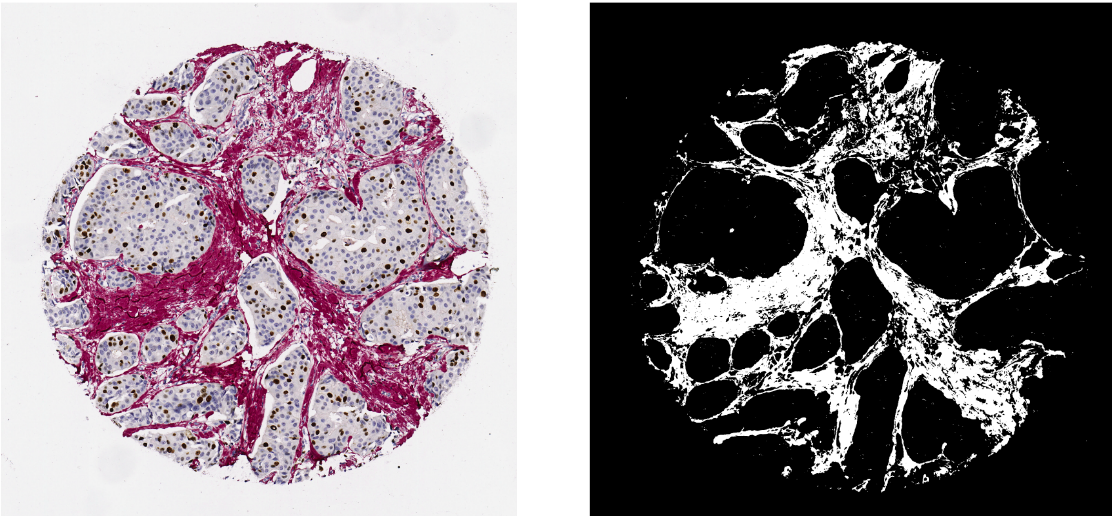
\includegraphics[width=\textwidth]{images/test.png}

\subsection{Features Generation}

After the collagen is extracted, the next step is to analyse it and compute
the features that can allow to diagnose the patients. More specifically, a
H\&E stained image is given corresponding to one patient. We wish to
inspect the image and predict the cancer severity stage for that person. The
following prediction pipeline is executed for this task:

\begin{itemize}
    
\item A collagen mask is computed from the image. For that the image is split
      into $256 \times 256$ tiles and the trained model is applied to each
      of the tile. The tiles are then merged into a single mask. Each cluster of
      connected pixels (using 8-connectivity [10]) that has less than 50 pixels is considered a
      noise and removed from the mask.

\item A skeletonization function [11] is applied on the mask. This transforms
      a white collagen regions into 1 pixel wide representations. The skeleton
      tree is chopped into individual edges and each edge gets assigned a
      unique id.

\item A breath first search algorithm [12] is then applied to find for each collagen
      pixel in the mask its closest skeleton edge. In this way the collagen
      is divided into regions and for each region we can compute its
      features.

\item For each region we compute 16 statistics and average them over all regions. The statistics
      include region length (computed as the number of pixels in the corresponding skeleton 
      edge), width (computed as the total number of pixels in the region divided by length),
      collagen to area ratio (computed as the total number of pixels in the region divided by
      the area of the smallest rectangle enlosing the region) and 13 haralick parameters
      (excluding the 14th due to its instability) [13,14]. We then use these parameters as
      features to predict the severity stage of cancer for each patient.

\end{itemize}


\subsection{Diagnosis prediction \& Results}

The section above gives multiple features (i.e. a list of numerical values) for
each H\&E stained image. The final step is to use this feature list to predict
the outcome. In this study we used two cohorts for outcome prediction, each cohort
acquired from the National Center of Pathology, Vilnius. 

The first cohort comprises 25 large H\&E stained images (e.g. $57767 \times 45287$ pixels),
each image per patient. 6 of them are related with the positive outcome, 19 with the negative.
We first compute the 16 statistics mentioned above for each of the patients. To obtain results
for this dataset, we perform the Kaplan-Meier analysis [15] on the cohort. For each of the 16
computed features (i.e. a vector of 25 numbers, one vector per feature) we use a Cutoff finder
package [16, 17] to derive a threshold for that feature. We then plot two Kaplan-Meier curves
based on the threshold: one for numbers less than the threshold, the other for numbers higher
than the threshold. We obtain 16 plots in this way:

  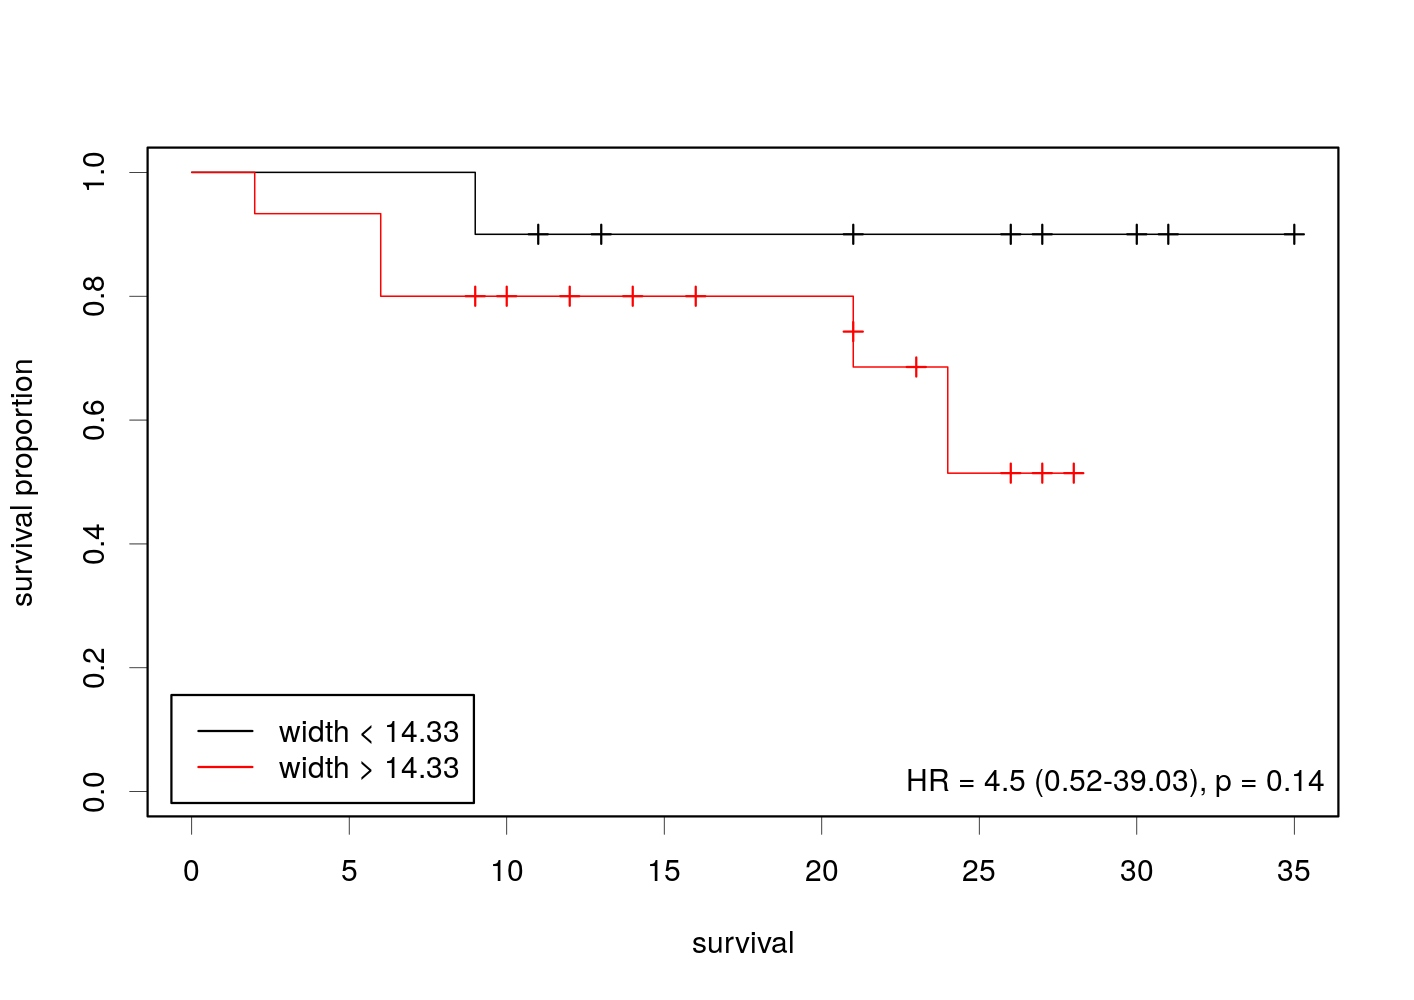
\includegraphics[width=65mm]{plots/width.jpg} 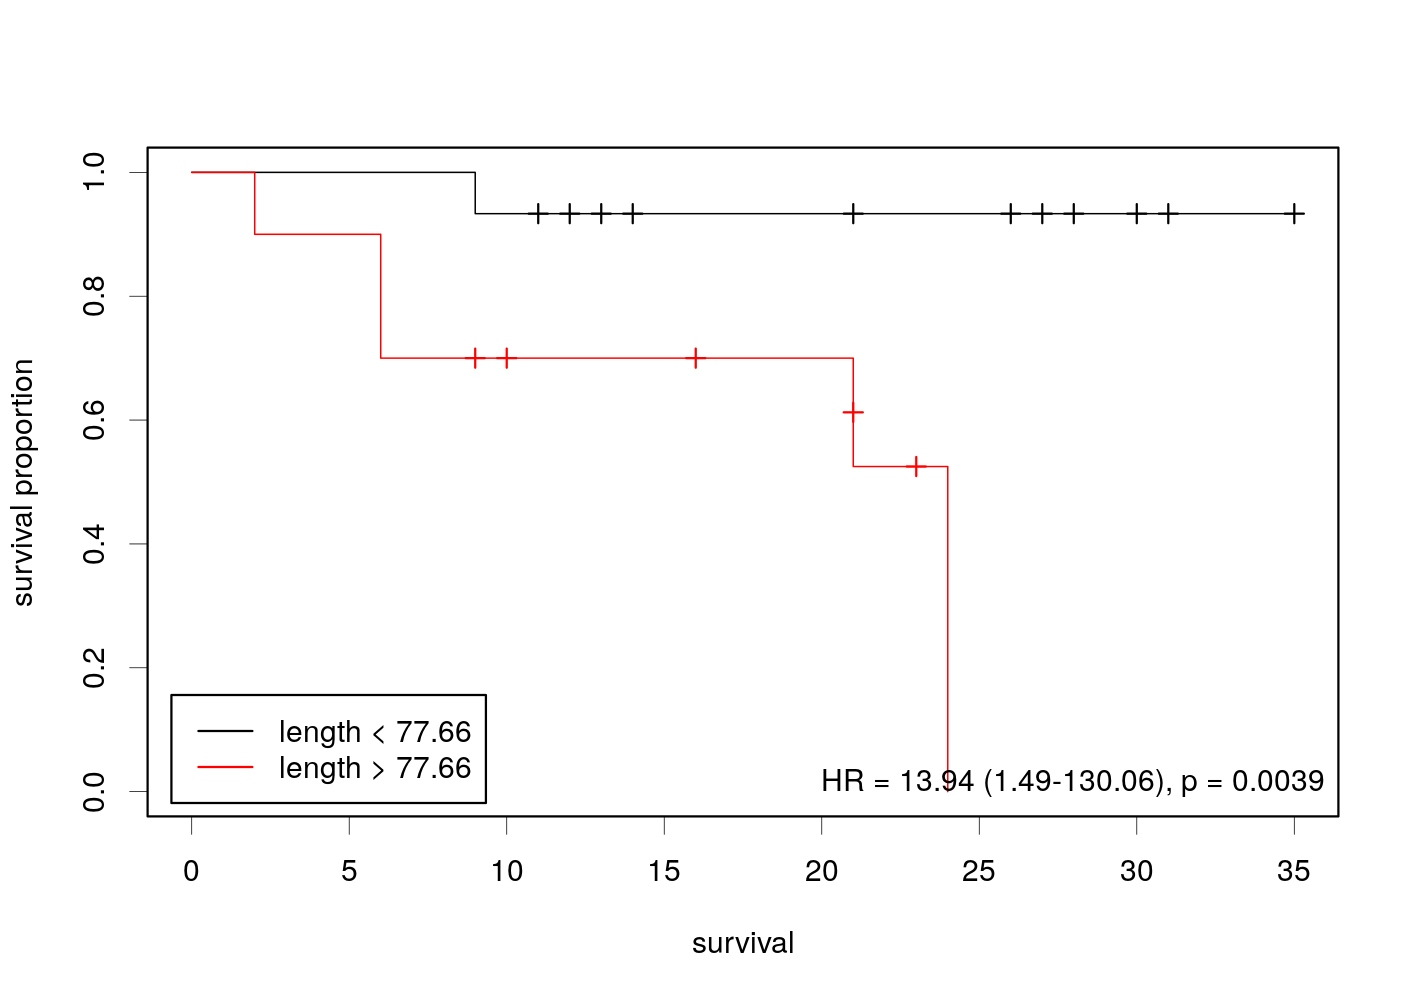
\includegraphics[width=65mm]{plots/length.jpg} \\
  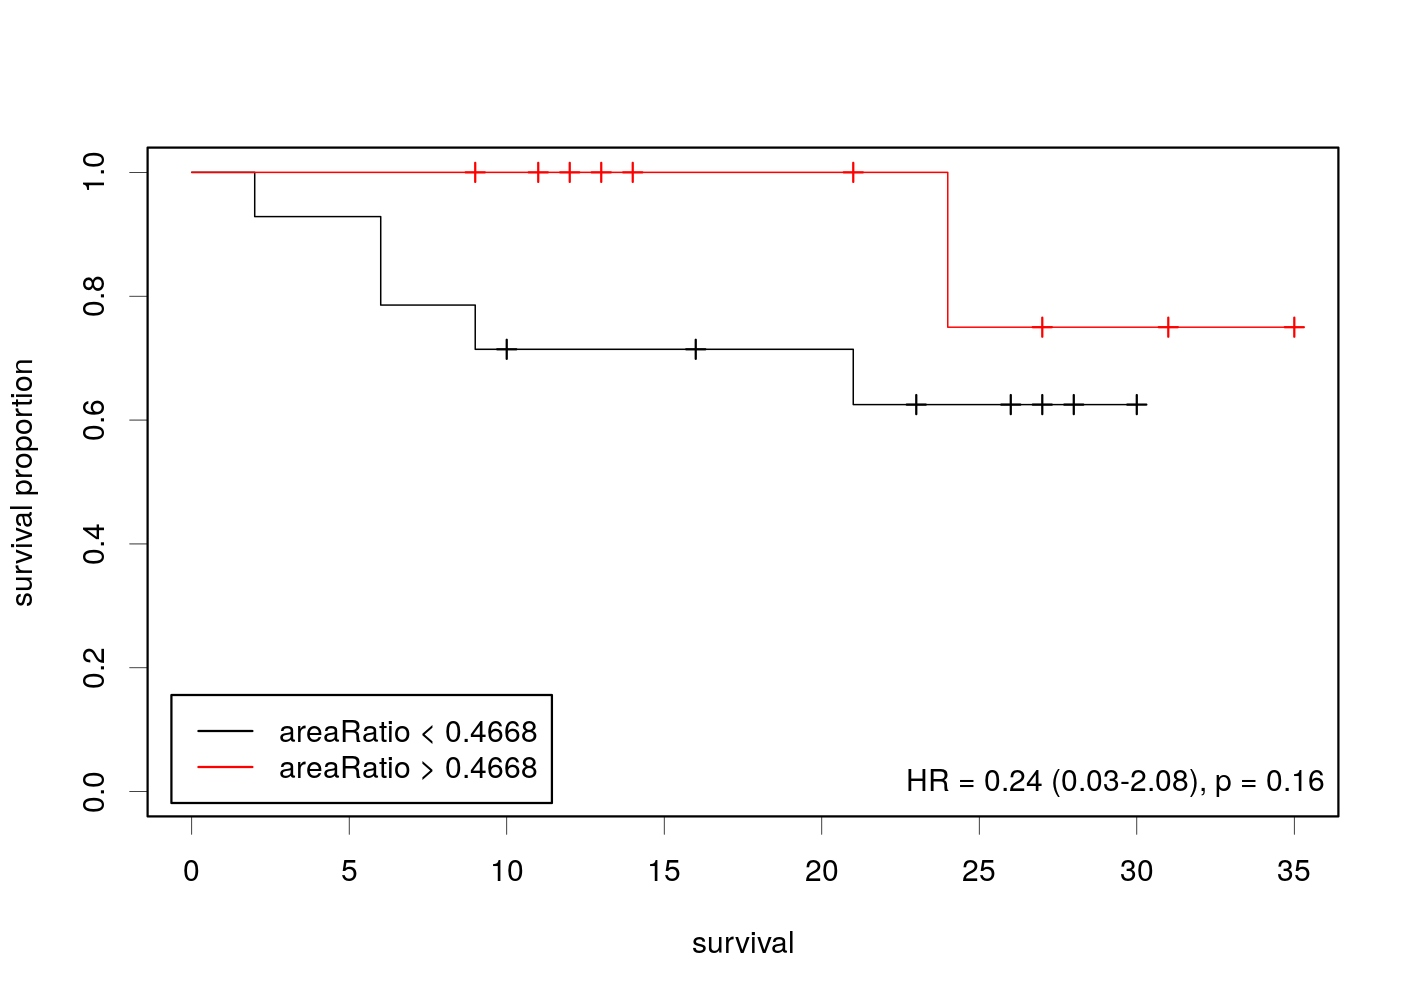
\includegraphics[width=65mm]{plots/ratio.jpg} 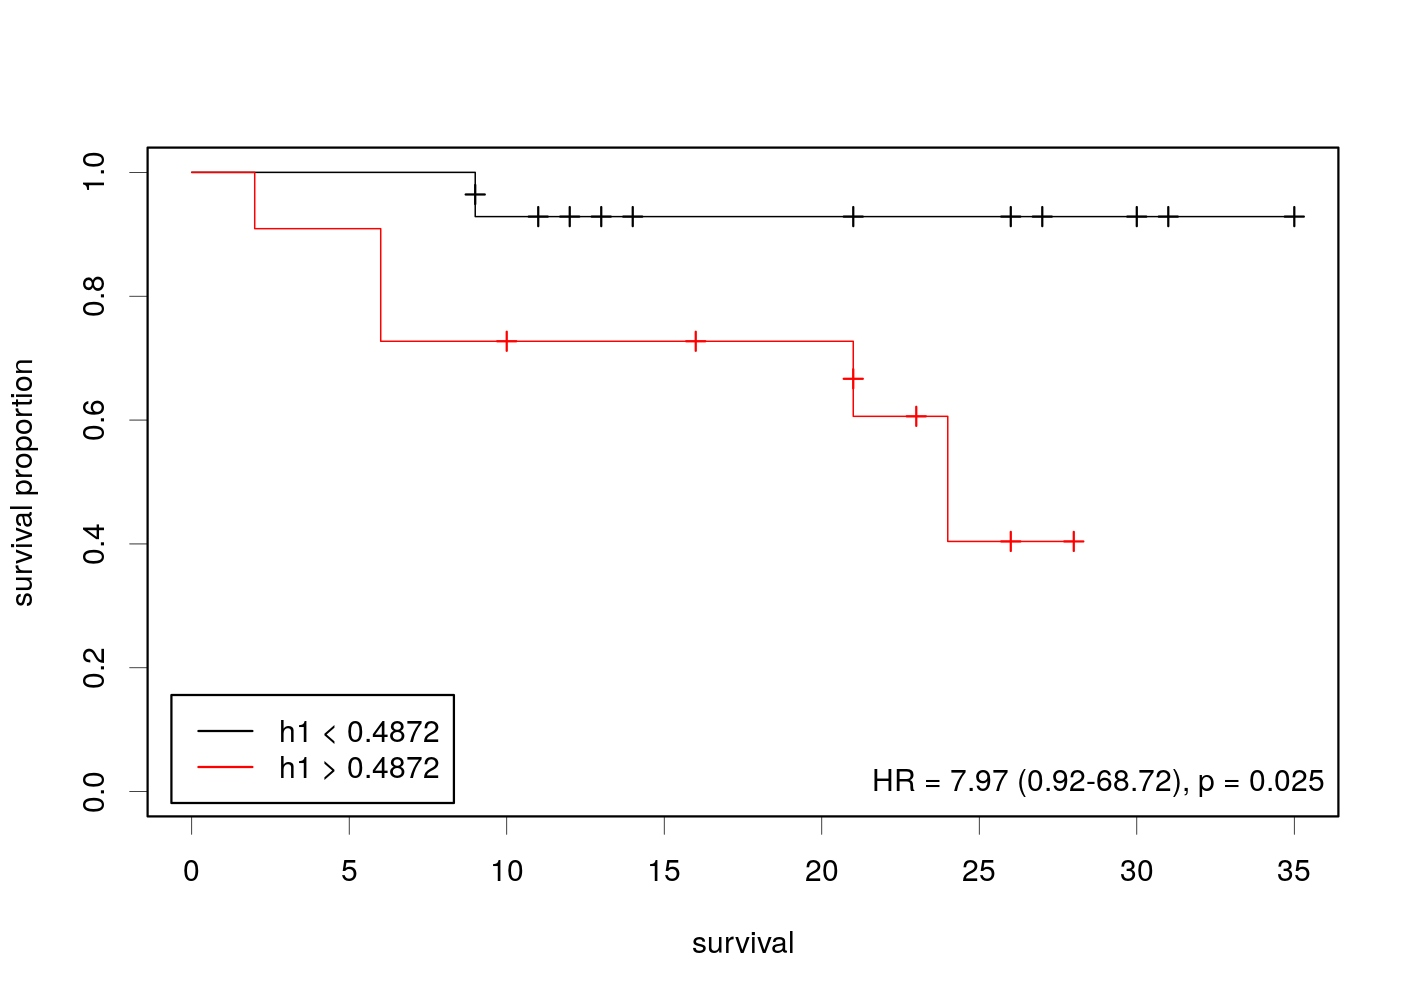
\includegraphics[width=65mm]{plots/h1.jpg} \\
  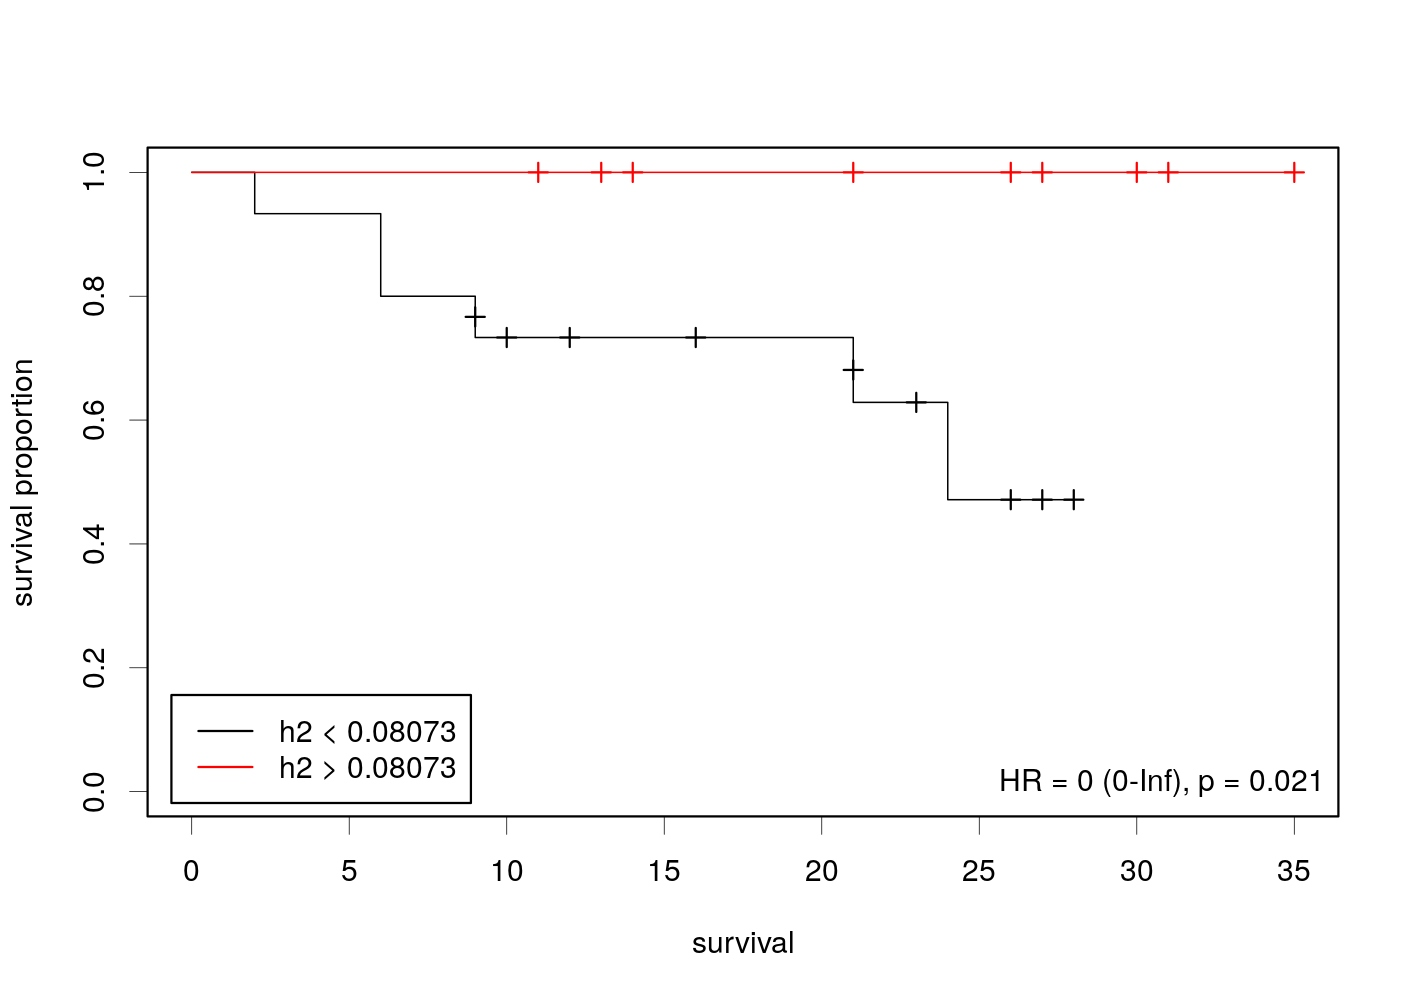
\includegraphics[width=65mm]{plots/h2.jpg} 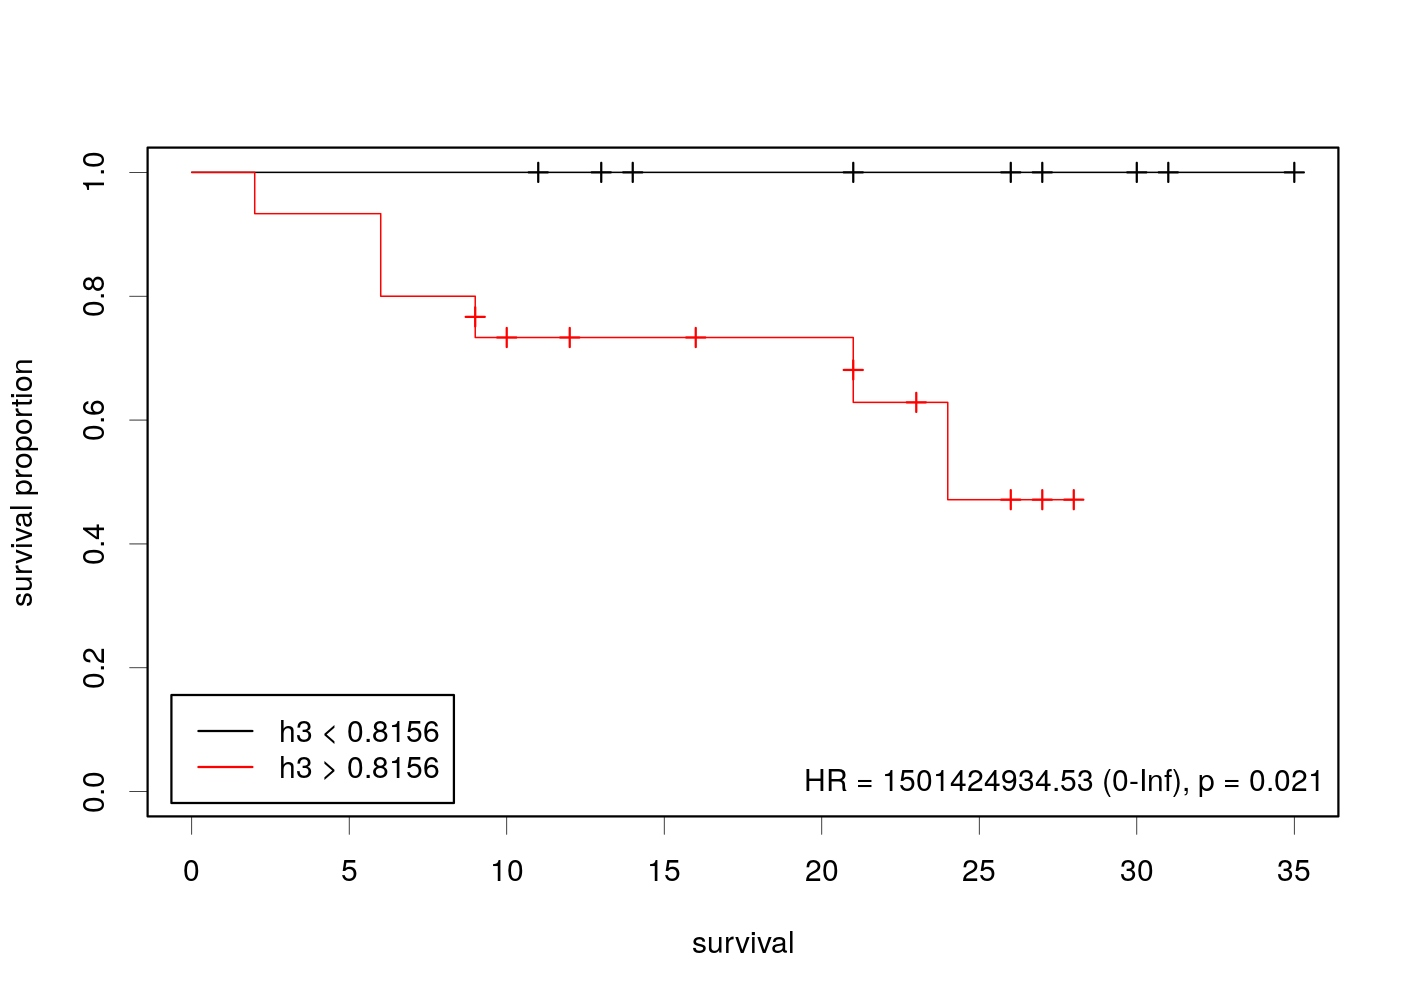
\includegraphics[width=65mm]{plots/h3.jpg} \\
  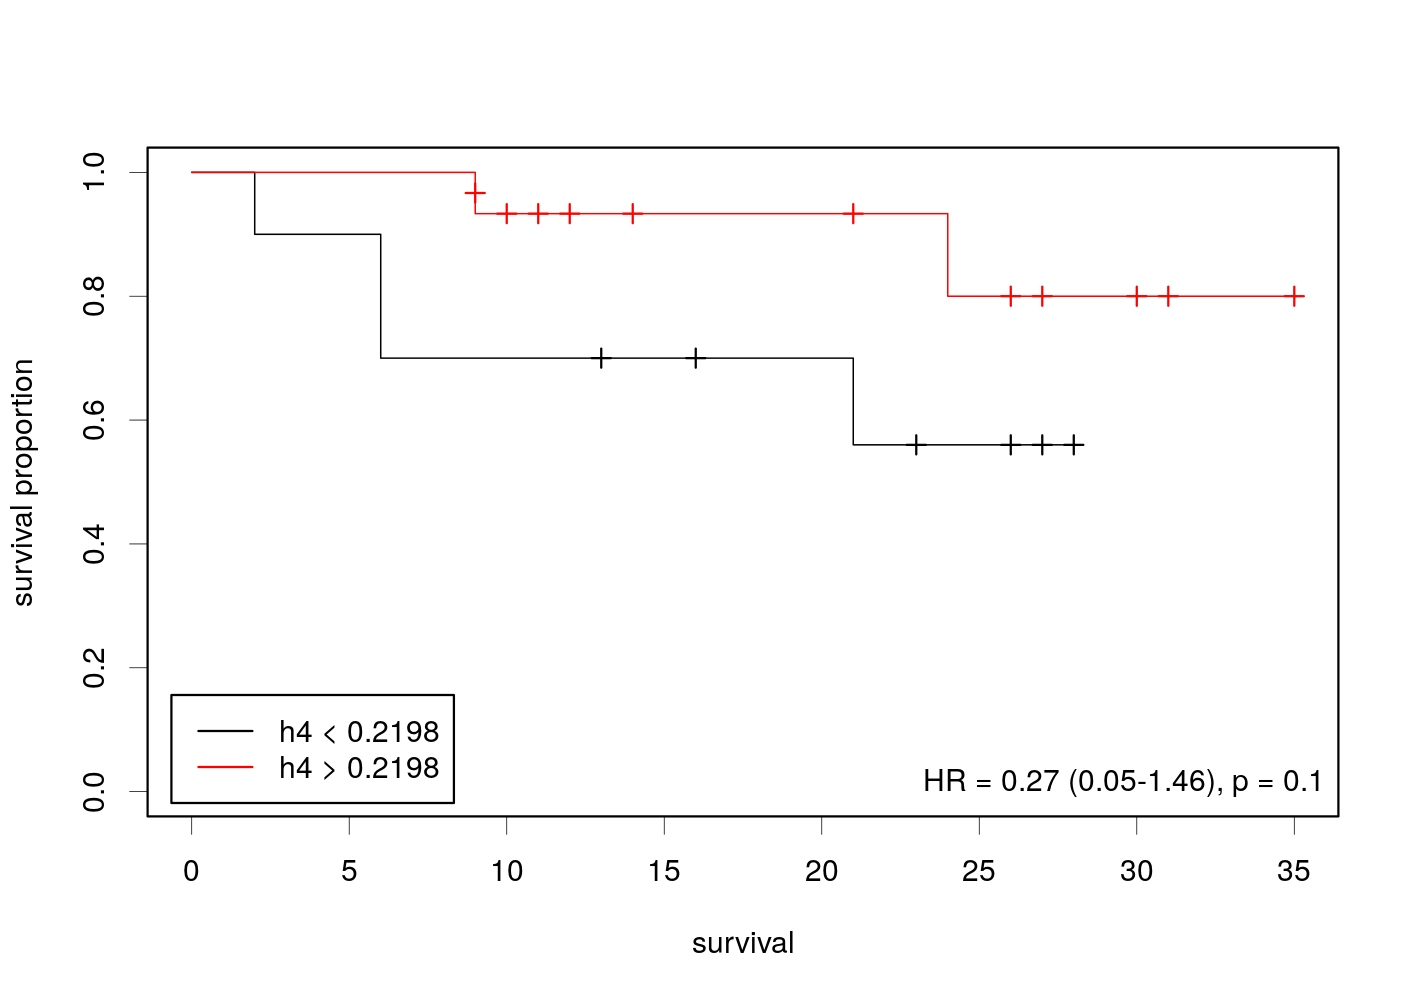
\includegraphics[width=65mm]{plots/h4.jpg} 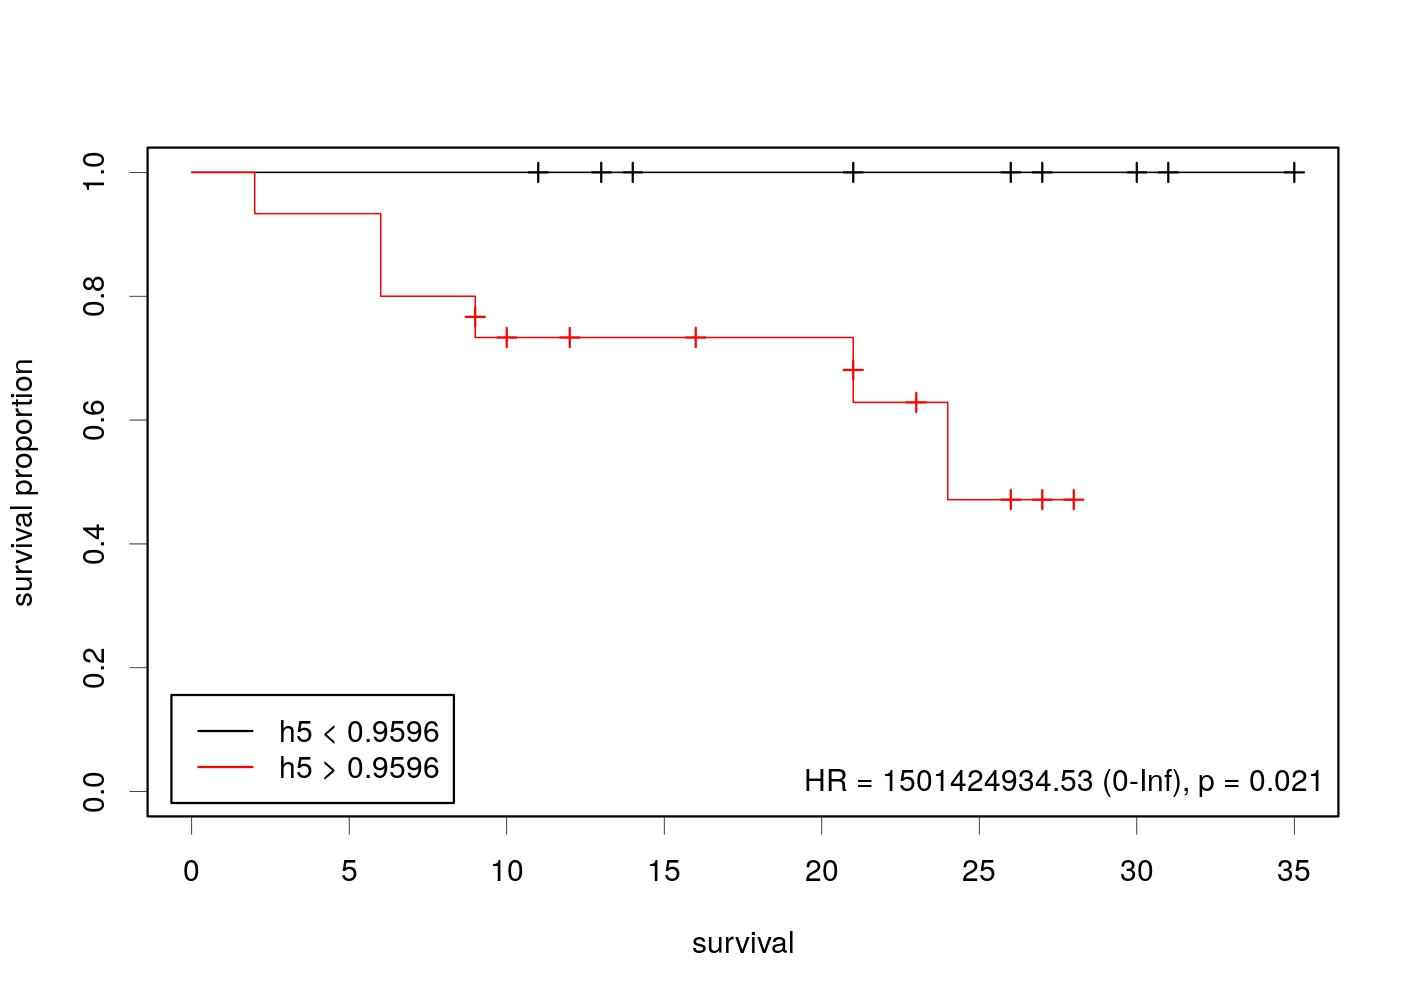
\includegraphics[width=65mm]{plots/h5.jpg} \\
  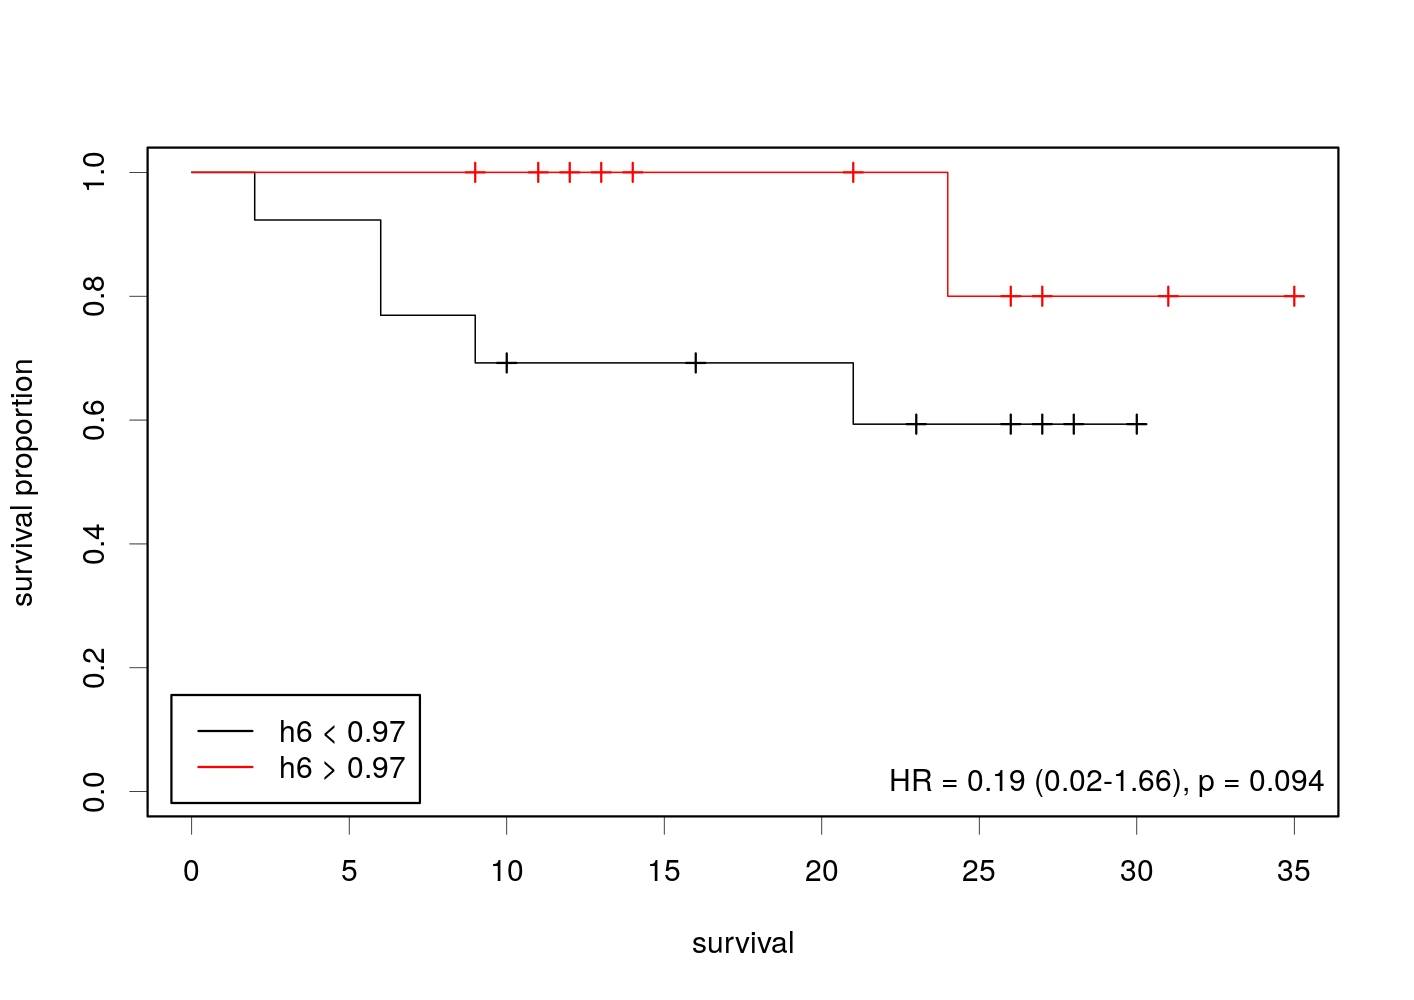
\includegraphics[width=65mm]{plots/h6.jpg} 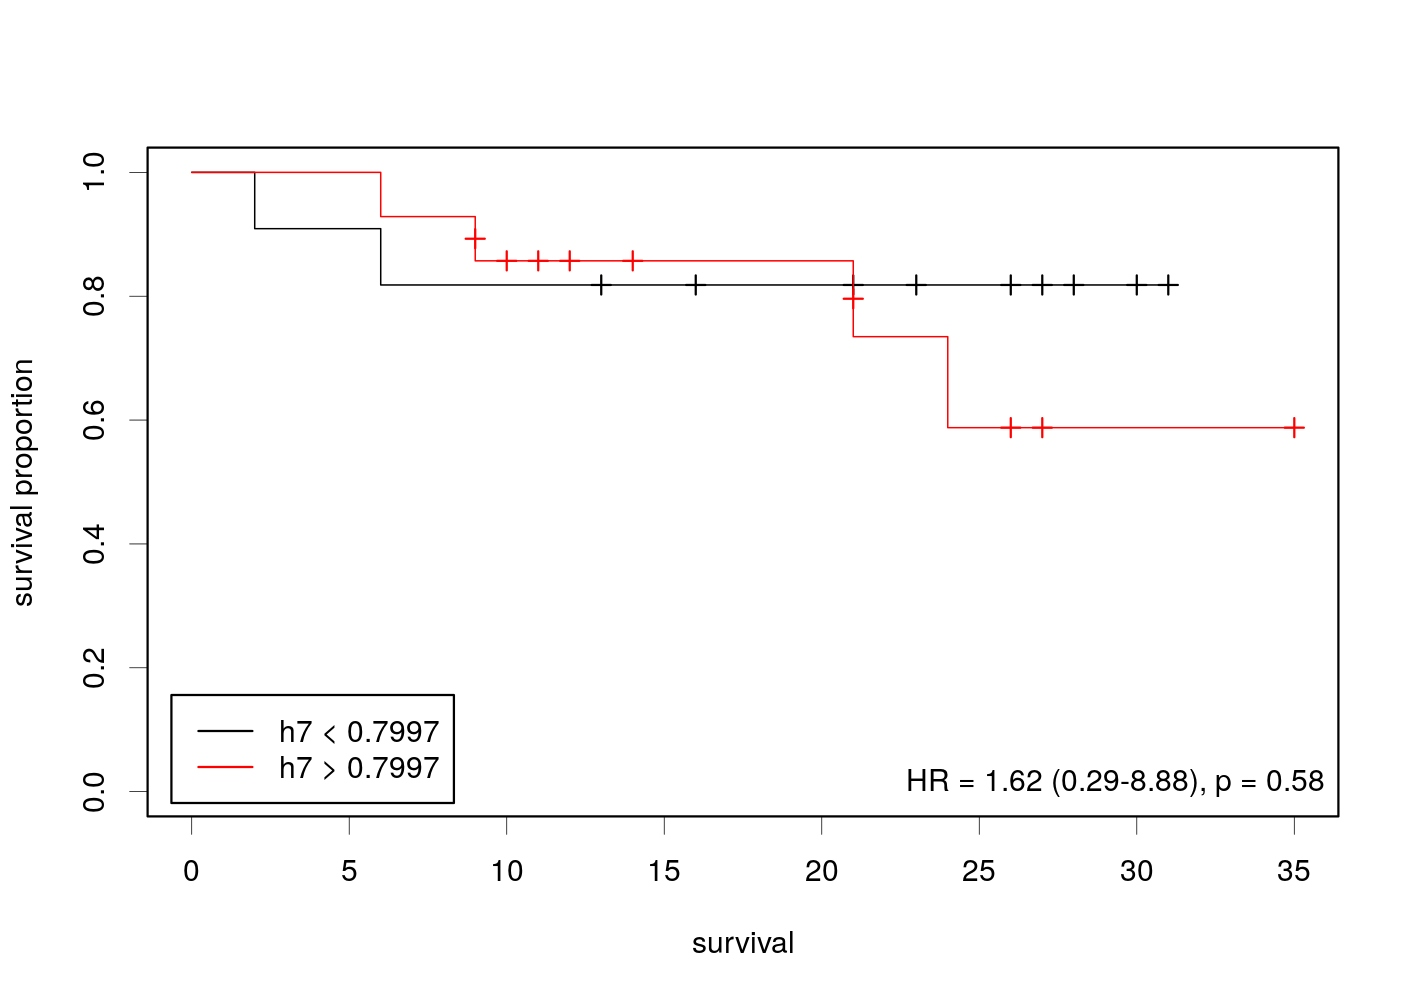
\includegraphics[width=65mm]{plots/h7.jpg} \\
  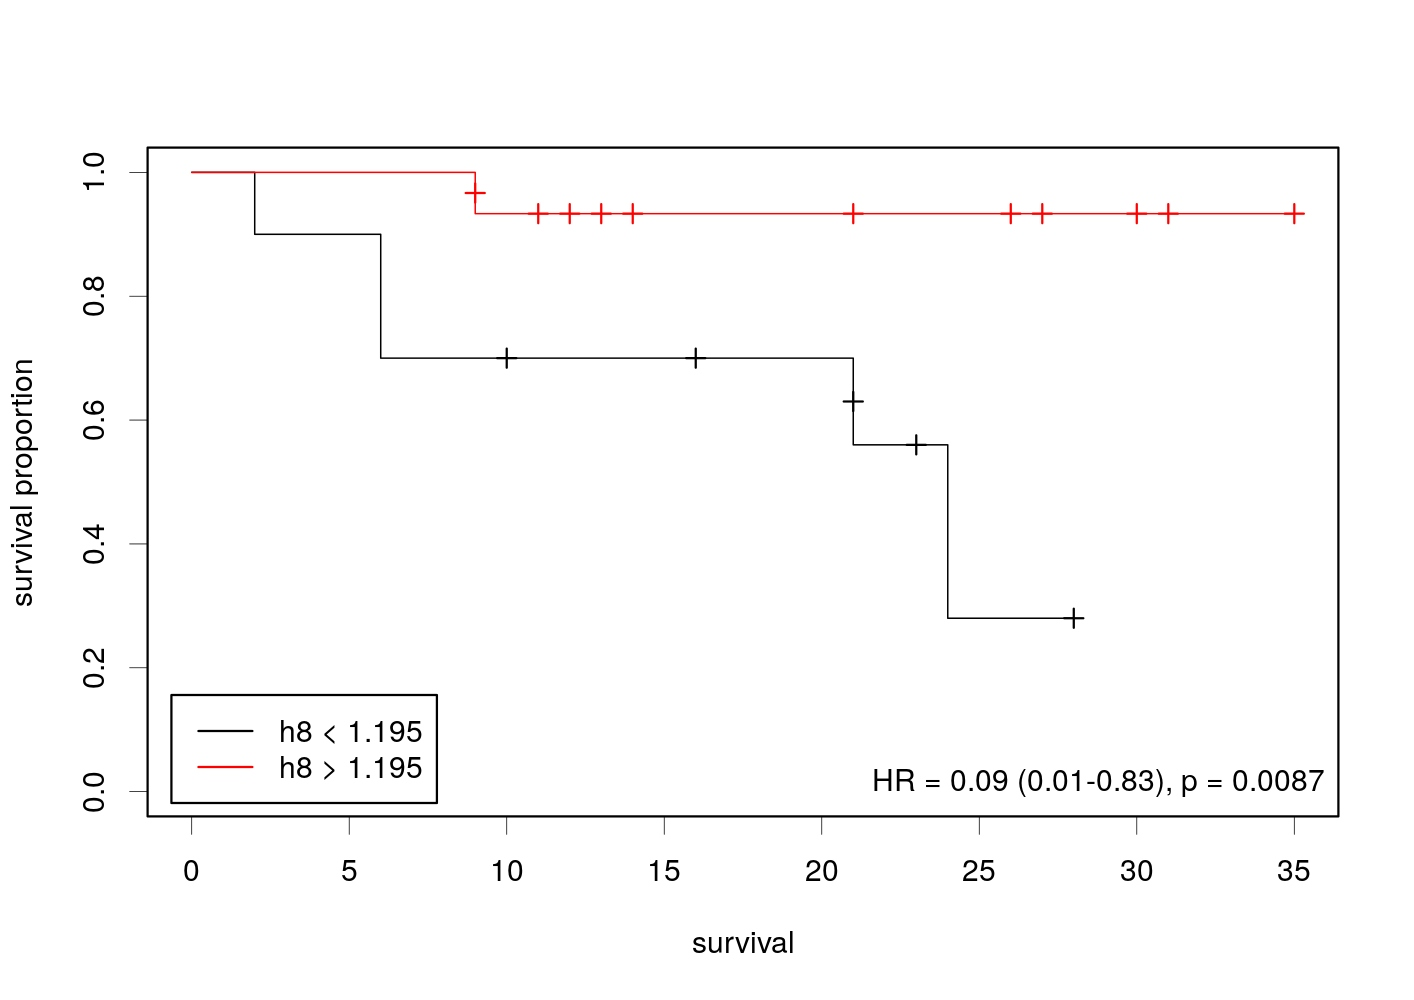
\includegraphics[width=65mm]{plots/h8.jpg} 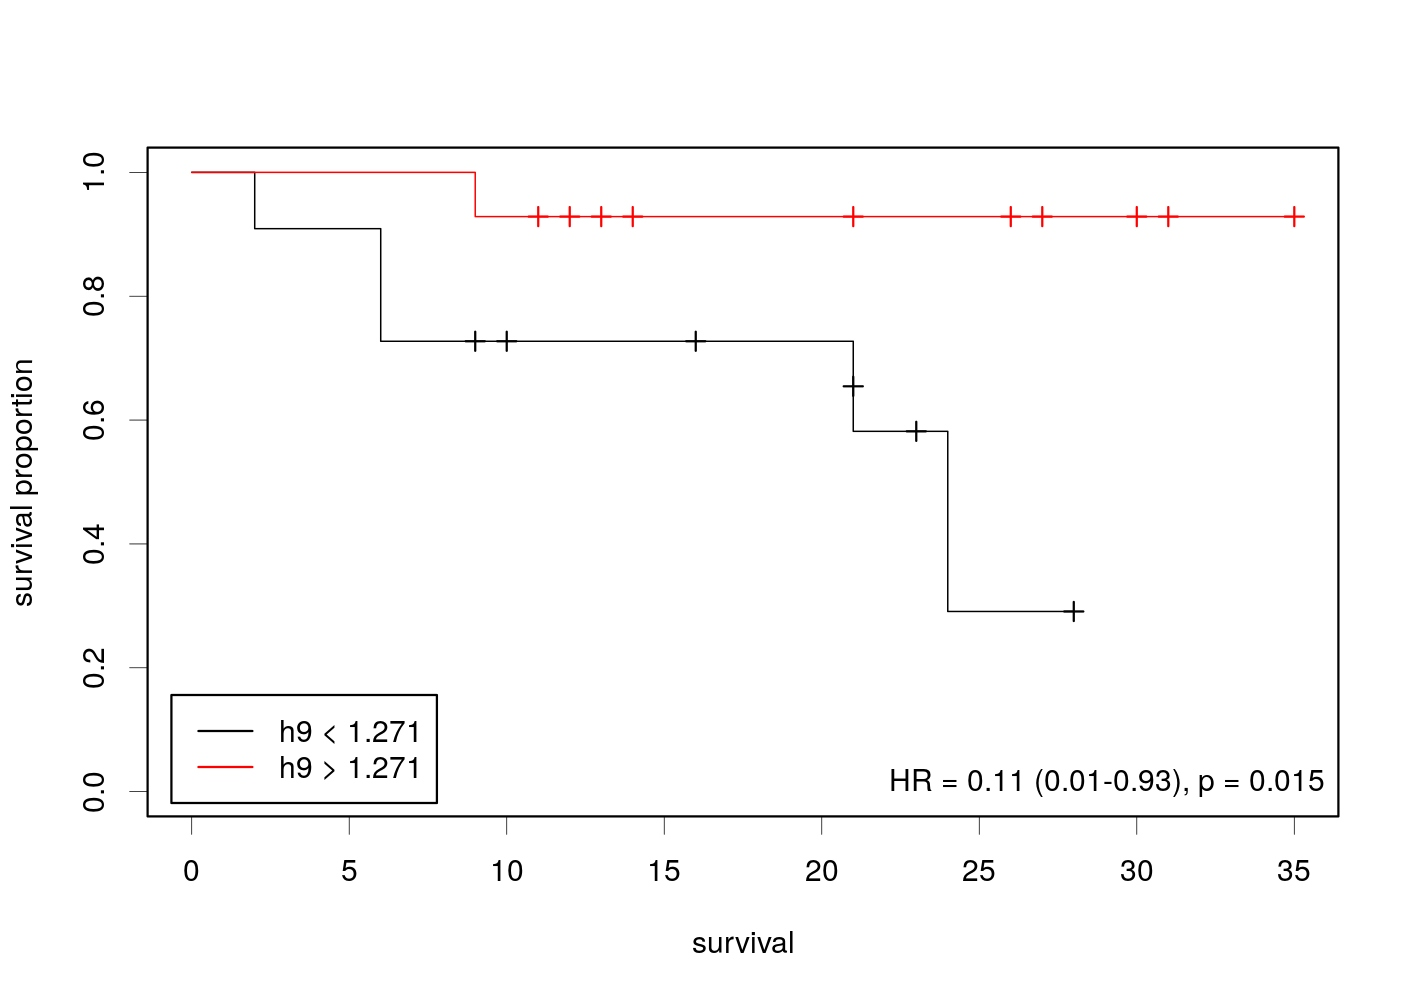
\includegraphics[width=65mm]{plots/h9.jpg} \\
  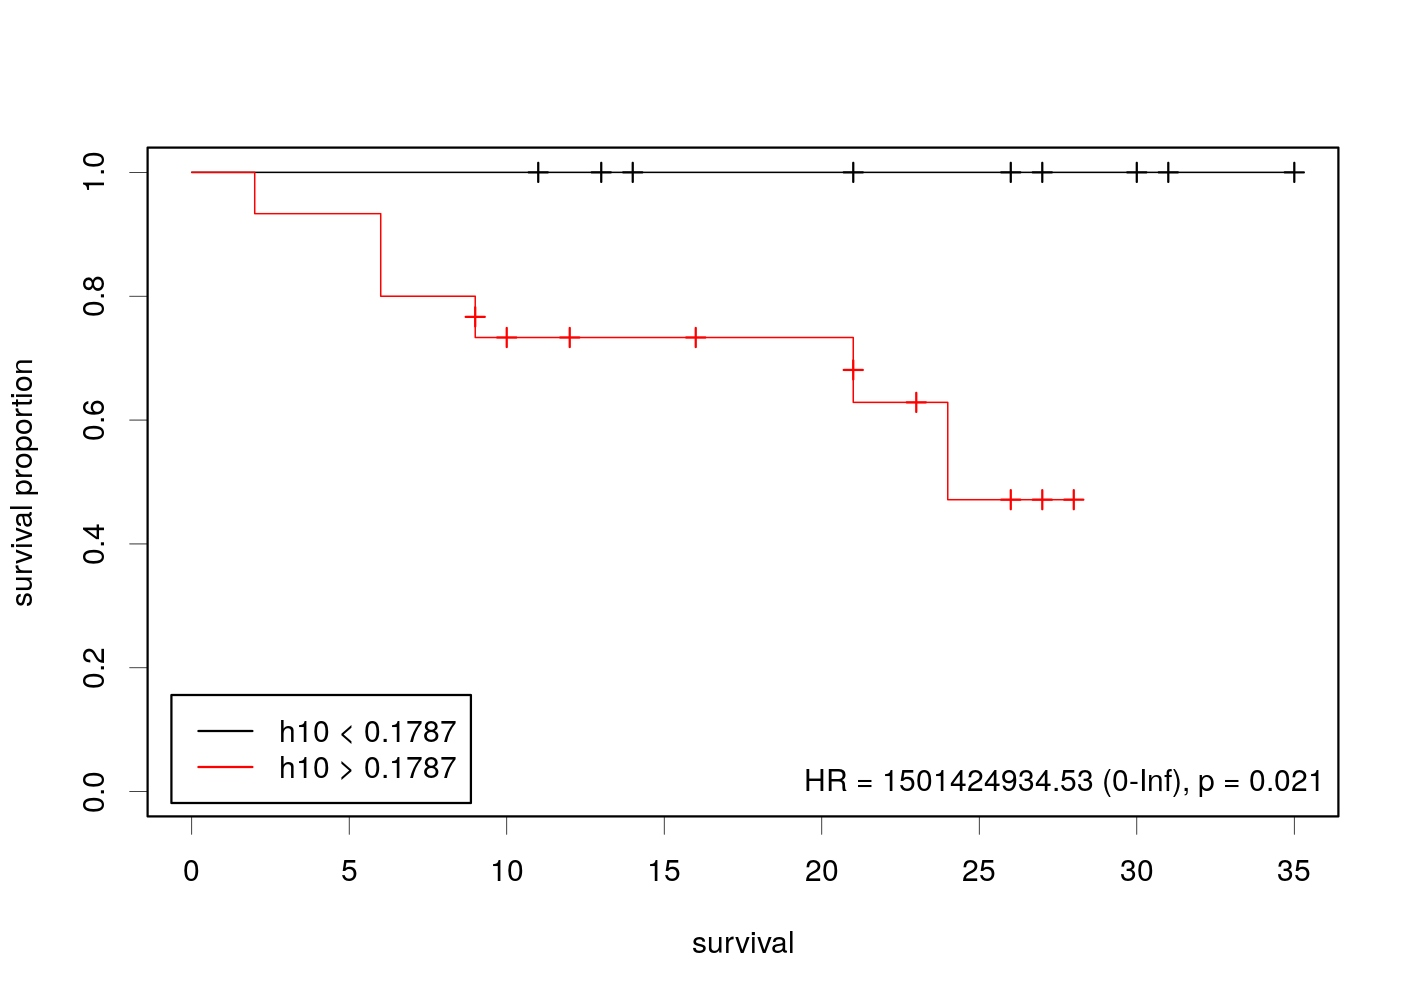
\includegraphics[width=65mm]{plots/h10.jpg} 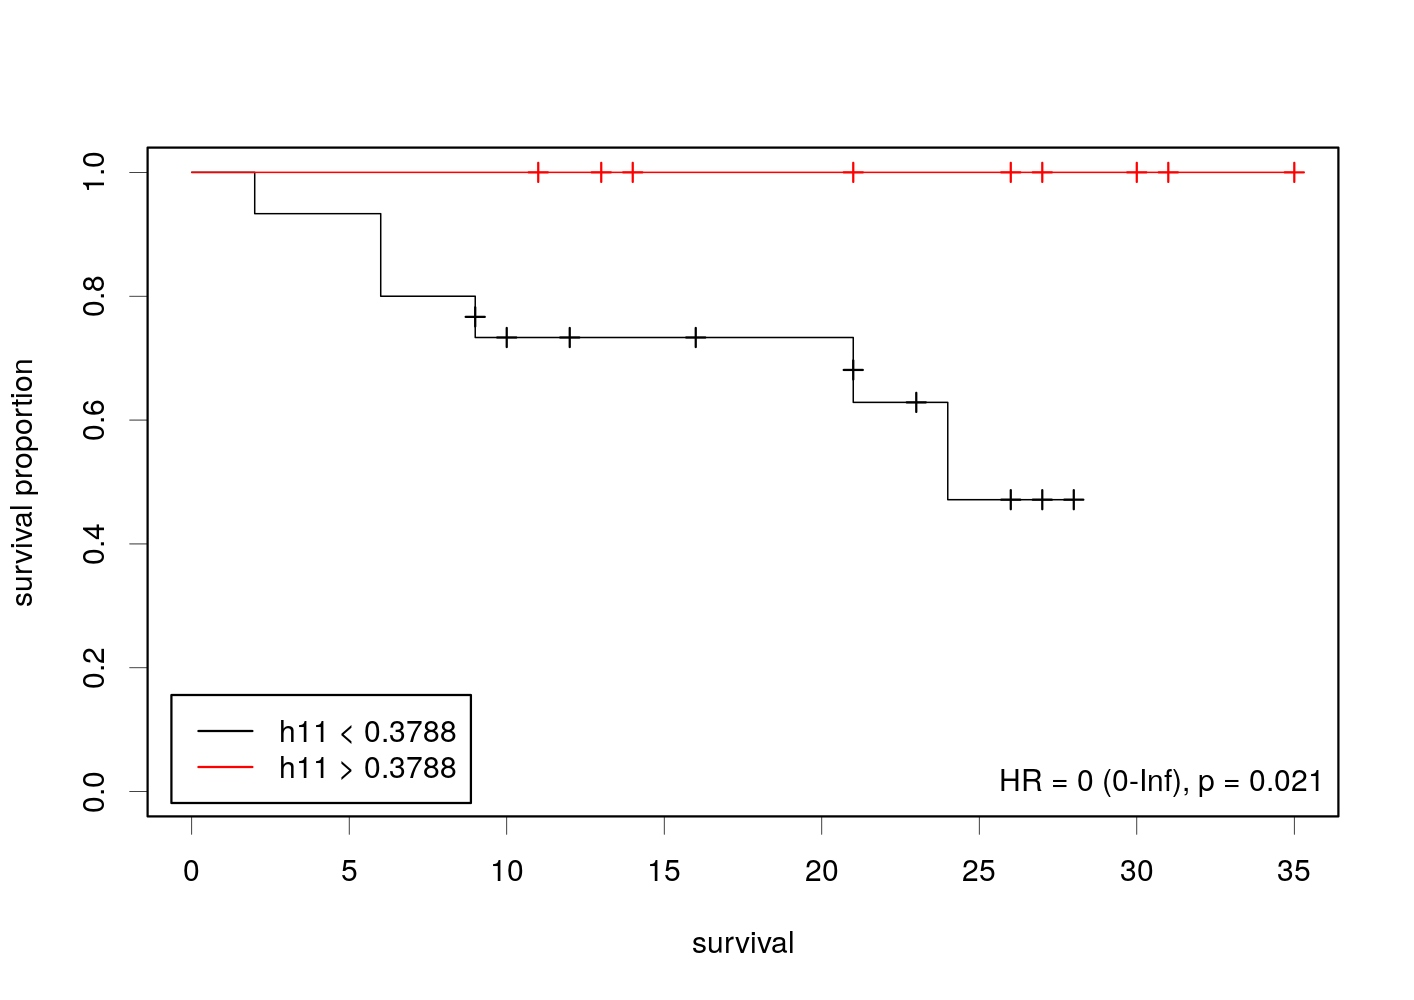
\includegraphics[width=65mm]{plots/h11.jpg} \\
  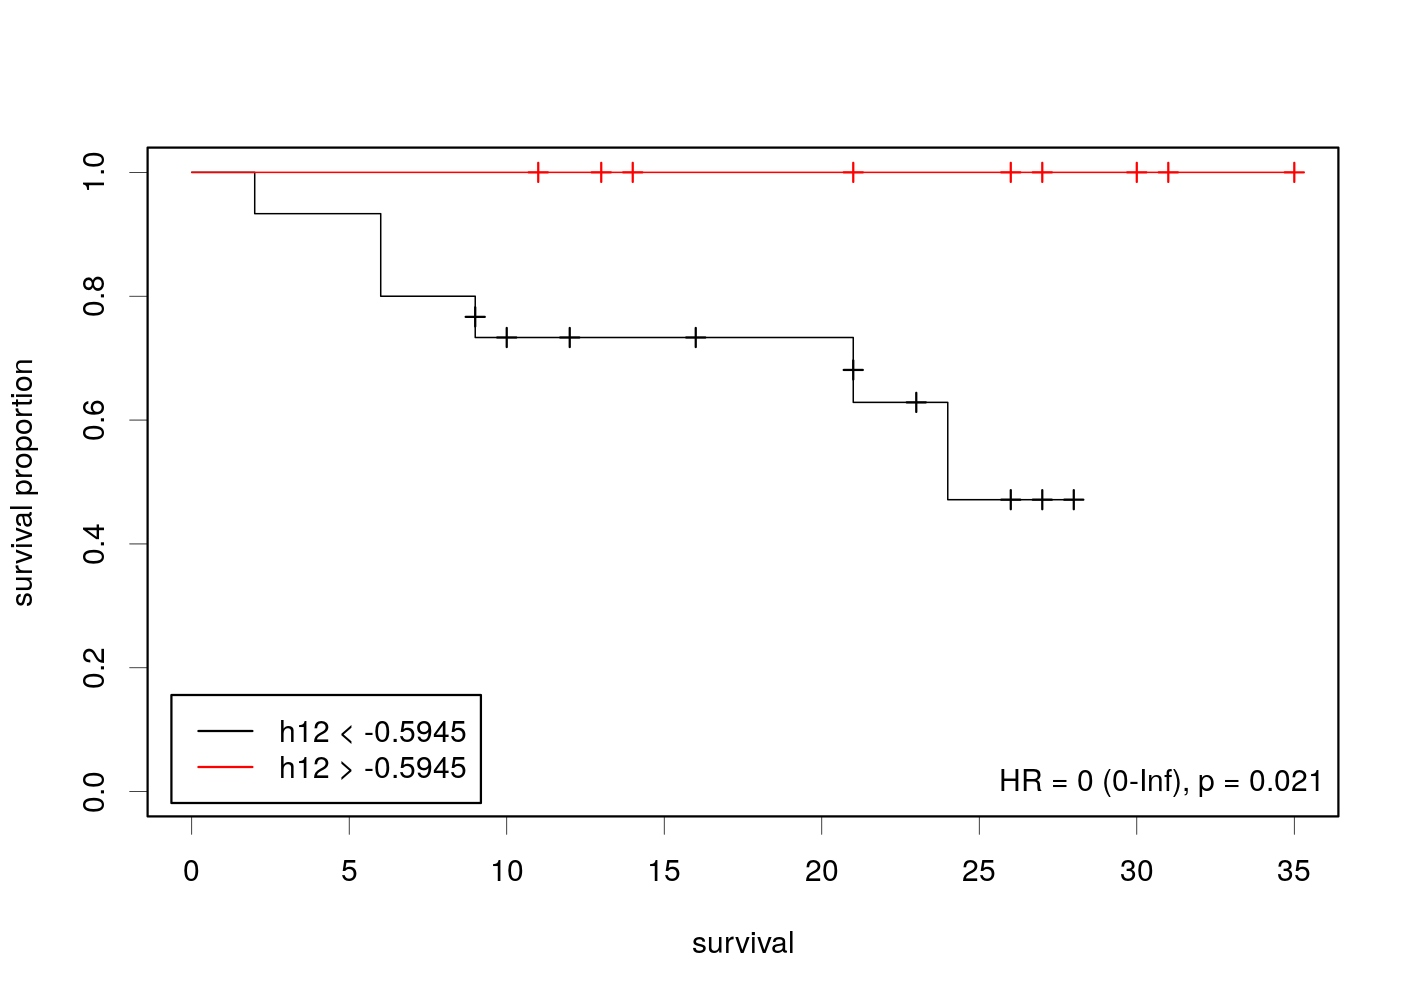
\includegraphics[width=65mm]{plots/h12.jpg} 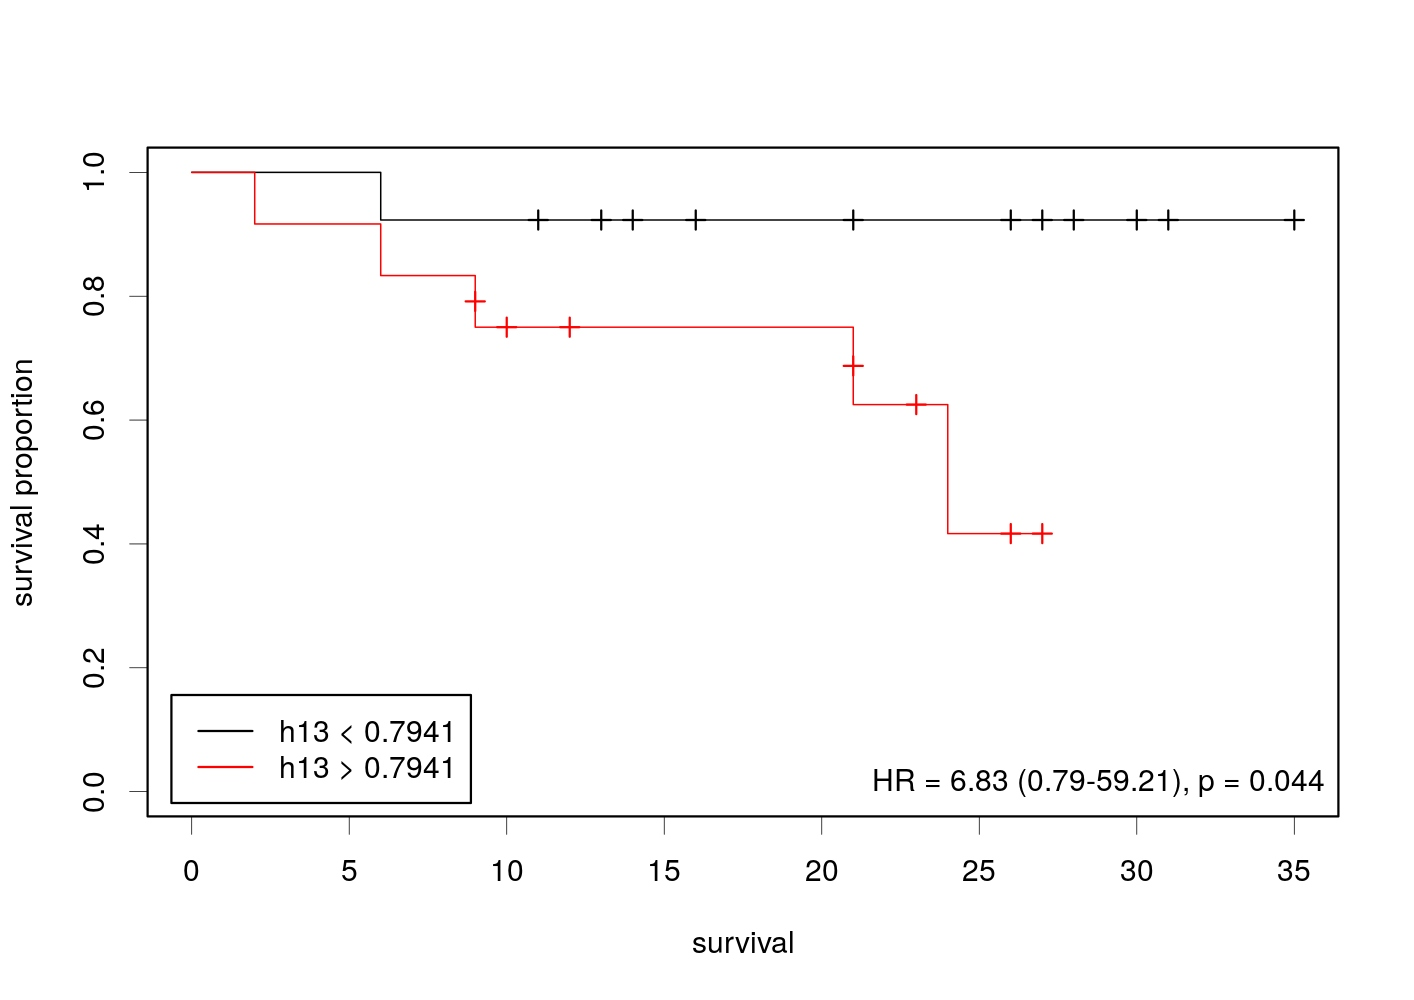
\includegraphics[width=65mm]{plots/h13.jpg} \\

11 of these plots (length, h1, h2, h3, h5, h8, h9, h10, h11, h12, h13) report significant
p-value scores (less than 5\%).

The second cohort comprises 92 TMA spots [18] of size $1500 \times 1500$, each spot per patient.
71 of them are related with the positive outcome, 21 with the negative. Firstly, we apply the
same Kaplan-Meier analysis on the second cohort. No significant features are found in this set.

However, the larger size of this cohort allows us to apply a more sophisticated statistical
technique to generate predictions. We augment the data by taking 21 negative images and rotating
them by 90, 180 and 270 degrees. This increases the size of the dataset up to $84+71=155$ samples.
We compute 16 features for each sample as before. We then split the data into training and test
sets. We train a binary classification model on the training data (a neural network with 2 dense
hidden layers of 128 nodes each was chosen) and evaluate it on the test data. We report 51\%
accuracy on the test set.

The relatively small size of images ($1500 \times 1500$) allows us to try one more approach. We
build a second convolutional neural network that takes the whole image as an input. The
convolutional neural network has multiple convolution + max pooling layers followed by a pair of dense layers that return a binary output. We again train and evaluate the CNN on a train/test split.
We report 54\% accuracy on the test set. 

\section{Conclusions}

    The study results showed that the visual pattern of the H\&E stained collagen
    in the tissue is too complex for a simple neural network to infer a useful signal
    for generating a diagnosis prediction. This suggests that to automate the task of predicting
    a diagnosis from an image, an add-hoc patterns recognised by expert pathologists need to be
    incorporated into the prediction pipeline.

\section{References}

\begin{enumerate}

\item H\&E stain. https://en.wikipedia.org/wiki/H\%26E\_stain

\item Provenzano PP, Eliceiri KW, Campbell JM, Inman DR, White JG, Keely PJ. Collagen reorganization at the tumor-stromal interface facilitates local invasion. BMC Med. 2006;4:38.

\item Provenzano PP, Eliceiri KW, Yan L, Ada-Nguema A, Conklin MW, Inman DR, et al. Nonlinear optical imaging of cellular processes in breast cancer. Microsc Microanal. 2008;14:532–48.

\item Provenzano PP, Inman DR, Eliceiri KW, Knittel JG, Yan L, Rueden CT, et al. Collagen density promotes mammary tumor initiation and progression. BMC Med. 2008;6:11.

\item Conklin MW, Eickhoff JC, Riching KM, Pehlke CA, Eliceiri KW, Provenzano PP, et al. Aligned collagen is a prognostic signature for survival in human breast carcinoma. Am J Pathol. 2011;178:1221–32.

\item Provenzano PP, Inman DR, Eliceiri KW, Trier SM, Keely PJ. Contact guidance mediated three-dimensional cell migration is regulated by Rho/ROCK-dependent matrix reorganization. Biophys J. 2008;95:5374–84.

\item Jeremy S. Bredfeldt, Kevin W. Eliceiri1. Automated quantification of aligned collagen for human breast carcinoma prognosis. J Pathol Inform, 2014;

\item Olaf Ronneberger, Philipp Fischer, Thomas Brox. U-Net: Convolutional Networks for Biomedical Image Segmentation. Medical Image Computing and Computer-Assisted Intervention (MICCAI), 2015.

\item Python Keras API. https://keras.io/

\item Pixel connectivity types. https://en.wikipedia.org/wiki/Pixel\_connectivity

\item Skeletonization function.
      
      https://scikit-image.org/docs/dev/auto\_examples/edges/plot\_skeleton.html

\item Breath-first search algorithm: https://en.wikipedia.org/wiki/Breadth-first\_search

\item Haralick features definition.
      
      http://murphylab.web.cmu.edu/publications/boland/boland\_node26.html

\item Haralick features in python. https://mahotas.readthedocs.io/en/latest/features.html

\item Kaplan-Meier estimator. https://en.wikipedia.org/wiki/Kaplan--Meier\_estimator

\item Jan Budczies, Carsten Denkert. Cutoff Finder: A Comprehensive and Straightforward Web Application Enabling Rapid Biomarker Cutoff Optimization, 2012.

\item Cutoff Finder software. http://molpath.charite.de/cutoff/

\item Tissue microarray. https://en.wikipedia.org/wiki/Tissue\_microarray

\end{enumerate}


\end{document}
